\chapter{Requirements gathering} \label{chap:ReqEng}

This chapter determines which requirements the artifact must meet to solve the problem. Following the relevance cycle as presented in \ref{topic:relevance cycle}, the process of gathering the requirements for the solution gives additional insights into the problem space, which in turn helps define the solution and the requirements the artifact must meet to solve the problem. The chapter discusses the methods (expert interviews and qualitative content analysis after Mayring) used to elicit the requirements. The process of requirements elicitation is described in more detail in appendix \ref{anhang:ReqEng}. In the ensuing sections, the data is collected in the form of expert interviews, the content is qualitatively analyzed, and existing approaches to solve this problem are investigated. These approaches serve as input for the following design process. Overall, this chapter lays the groundwork for the solution definition.

\section{Research method and objective}
Interviews present one example of conversational methods (described in appendix \ref{anhang:ReqEng}) and the most commonly used method to elicit information. An interview is defined as motivating the interviewee to share their information, opinion, attitude and knowledge regarding specific topics.\footcite[Cf.][p.133]{KrugerqualitativeInhaltsanalyseMethode2004} The statement of \cite{WhiteProbingunderstanding1992}, \enquote{[An] interview is the most direct method, among all the probes, of assessing a person’s understanding}, is supported by a great number of authors in the field,\footcites[Cf.][p.174]{MacaulayRequirementscapturecooperative1993}[cf.][p.105]{SommervilleSoftwareengineering2011}[cf.][p.25]{ZowghiRequirementselicitationsurvey2005}[cf.][p.172]{HickeyElicitationtechniqueselection2003}[cf.][p.227]{ZhangEffectiverequirementsdevelopmentA2007}[cf.][p.92]{MasonQualitativeresearching2002} because interviews not only allow the identification of facts and subjective opinions of the stakeholders by face to face conversation, but they also allow the discovery of conflicts or politics.\footcites[Cf.][p.2]{TiwariMethodologySelectionRequirement2017} The requirements may be extracted directly from the stakeholders' verbalized thoughts, and if needed, the conversation allows further queries to treat specific topics more thoroughly and to discover hidden requirements. Due to these characteristics, interviews are deemed the best approach to gather the requirements for the artifact.

Because interviews are popular and widely used, numerous variations have developed that may be categorized by different aspects. An interview may be closed/structured (pre-defined set of questions, looking for clear answers), semi-structured (a more flexible set of questions allowing the researcher to adapt/innovate) or open-ended/unstructured (a discussion to discover requirements together, stakeholder talks from their perspective).\footcites[Cf.][p.2]{TiwariMethodologySelectionRequirement2017}[cf.][pp.39]{EdwardsWhatqualitativeinterviewing2013} The two latter types present qualitative interviews, characterized by less structured information and more flexibility in conversation flow.\footcite[Cf.][p.13]{EdwardsWhatqualitativeinterviewing2013} These types of interviews are chosen for when the data is most feasibly generated by asking the stakeholders for their opinion and stances about particular topics.\footcite[Cf.][p.76]{MasonQualitativeresearching2002} One instance of qualitative interviews is the expert interview which the following paragraphs describe in more detail.


% The statement of \cite{WhiteProbingunderstanding1992}, \enquote{[An] interview is the most direct method, among all the probes, of assessing a person’s understanding}, is supported by a great number of authors in the field,\footcites[Cf.][p.174]{MacaulayRequirementscapturecooperative1993}[cf.][p.105]{SommervilleSoftwareengineering2011}[cf.][p.25]{ZowghiRequirementselicitationsurvey2005}[cf.][p.172]{HickeyElicitationtechniqueselection2003}[cf.][p.227]{ZhangEffectiverequirementsdevelopmentA2007}[cf.][p.92]{MasonQualitativeresearching2002} because they allow the identification of facts and subjective opinions of the stakeholders by face to face conversation, but also the discovery of conflicts or politics.\footcites[Cf.][p.2]{TiwariMethodologySelectionRequirement2017}

% Interviews were and remain the most commonly used approach to elicit information. An interview is defined as motivating the interviewee to share their information, opinion, attitude and knowledge regarding certain topics.\footcite[Cf.][p.133]{KrugerqualitativeInhaltsanalyseMethode2004} The requirements can directly be extracted from the stakeholders' verbalized thoughts and if needed, the conversation allows further queries to treat specific topics more thoroughly and discover hidden requirements. Due to these characteristics, interviews are deemed the best approach to gather the requirements for the artifact.

\subsection{Expert interviews} \label{subsec:ExpertInterviews}
An expert interview is a semi-structured interview used for explorative purposes. These purposes include 1) the orientation in a new field of research, 2) the collection of context information to complement other research methods, and 3) the development of a theory or typology by synthesizing knowledge from various experts.\footcite[Cf.][p.450]{PfadenhauerExperteninterviewGesprachauf2007} It gathers the expert's knowledge on their field of expertise and explicitly documents it.\footcites[cf.][p.172]{HickeyElicitationtechniqueselection2003} Although it is a complex, elaborate and time consuming method to generate data, it is applied in various fields of research due to the high quality of insights gained from the expert's knowledge.\footcites[Cf.][p.459]{PfadenhauerExperteninterviewGesprachauf2007}[cf.][p.442]{MeuserExpertInneninterviewsvielfacherprobt1991}[cf.][p.424]{BuberQualitativeMarktforschungKonzepte2007}[cf.][p.179]{Flickintroductionqualitativeresearch2009}[cf.][p.465]{MeuserExperteninterviewkonzeptionelleGrundlagen2009}[cf.][p.31]{BognerInterviewsmitExperten2014}
%The expert interview in itself may be categorized into four different types depending on the interview's purpose.

The explorative expert interview helps gain insights into the problem space, and thus allows the better definition of the problem and the generation of hypotheses on how to solve this problem.\footcite[Cf.][p.28]{BognerInterviewsmitExperten2014} The primary goals of this type of interviews are 1) to collect relevant information about the research environment and the problem space as well as 2) to discover the experts' opinion and attitudes regarding that problem.\footcite[Cf.][pp.28/29]{BognerInterviewsmitExperten2014} Therefore, this type of interview is well suited to gather the requirements for the artifact as well as to collect more information regarding the problem.

\paragraph{Experts} The status of an expert is a relational status, depending on the issue and approach taken in the study.\footcites[Cf.][p.179]{Flickintroductionqualitativeresearch2009}[cf.][p.444]{MeuserExpertInneninterviewsvielfacherprobt1991} An expert may be any person who has distinguished knowledge in a particular subject and thus acts as a body of authority on that particular field. This knowledge, whether it stems from practical experience or in-depth study, allows the clear identification of a problem space and the formulation of meaningful instructions for others to solve that problem.\footcites[Cf.][p.469]{MeuserExpertInneninterviewsvielfacherprobt1991}[cf.][p.467]{MeuserExperteninterviewkonzeptionelleGrundlagen2009}[cf.][p.179]{Flickintroductionqualitativeresearch2009}[cf.][p.451]{PfadenhauerExperteninterviewGesprachauf2007}[cf.][p.19]{BognerInterviewsmitExperten2014}

\paragraph{Compendium of questions} As suggested by Meuser and Nagel, a compendium of questions is used as the basis for the interview.\footcite[Cf.][p.472]{MeuserExperteninterviewkonzeptionelleGrundlagen2009} The compendium's purpose is to provide an orientation for the researcher while motivating the interviewee to speak freely. It serves as a guideline by reminding the researcher of the interview's purpose. It allows the researcher to prepare and structure the interview beforehand to gain enough competency about the interviewee's field of expertise to enable a productive conversation.\footcites[Cf.][p.472 et seqq]{MeuserExperteninterviewkonzeptionelleGrundlagen2009}[cf.][p.133]{KrugerMethodennaturwissenschaftsdidaktischenForschung2014}[cf.][p.431 et seq]{BognerInterviewsmitExperten2014}[cf.][p.123 et seqq]{NiebertLeitfadengestutzteInterviews2014}[cf.][p.421]{AghamanoukjanQualitativeInterviews2007}
To ensure that the compendium may be applied effectively, it should be clear (open layout), not overloaded (limited number of questions), logically structured (questions are in a thematic order), use appropriate language (both conversational partners must understand each other), and serve as a guide (not restrictive).\footcite[Cf.][p.126]{NiebertLeitfadengestutzteInterviews2014}

The process of interviewing an expert is presented figure \ref{fig:InterviewProcess}. The process starts with the collection of all research questions and hypotheses regarding the study (step 1). The main research questions the study aims to resolve are divided into smaller questions, which are subsequently sorted and grouped by topic (step 2). Following the requirements outlined above, a subset of questions is put in the compendium (step 3). After that, the effectiveness and utility of the developed catalog of questions is tested by conducting a test interview beforehand and ensuring that the asked questions reflect the initial research questions. The compendium is hence refined iteratively until it is deemed appropriate for actual use (step 4). Once the compendium is completed, the experts to be interviewed are chosen (step 5). The selection of these experts depends on various factors, ranging from the subject of study, the quality of data, the study design to the availability of possible respondents.\footcites[Cf.][p.134]{KrugerqualitativeInhaltsanalyseMethode2004}[cf.][p.1 et seq.]{MorseDeterminingsamplesize2000}[cf.][p.137]{Flickintroductionqualitativeresearch2009} Then, the interviews are conducted in an open manner to entice an interesting and meaningful conversation (step 6) and are finally transcribed and analyzed (step 7). The analysis may focus on quantitative and qualitative information (or both) to extract useful information from the conversation.\footcites[Cf.][p.37 et seqq]{BognerInterviewsmitExperten2014}[cf.][p.454 et seqq]{MeuserExperteninterviewkonzeptionelleGrundlagen2009}[cf.][p.72]{MasonQualitativeresearching2002} Depending on the method of content analysis chosen, this step is divided into further activities.\footnote{For more information, see \ref{subsec:Mayring}}

\begin{figure}
    \centering
    \includesvg[width=\textwidth]{graphics/InterviewProcess}
    \caption[The interview process]{The interview process\protect\footnotemark}
    \label{fig:InterviewProcess}
\end{figure}

\footnotetext{With changes taken from \cite{MasonQualitativeresearching2002}, p.72}

The methodological analysis of the conducted interviews is essential to extracting the needed information from the conversation. However, the process does not define an exact instruction on how to perform this analysis. For this purpose, the method of qualitative content analysis after Mayring is chosen/consulted, which is described in the following subsection.

\subsection{Qualitative content analysis} \label{subsec:Mayring}
A methodological approach to evaluate the conducted interviews is key to ensure the correctness and completeness of the information. Since the purpose of the interviews is to collect qualitative data and not to compare the key messages from each expert with one another, a qualitative method is appropriate to generate a general statement regarding the requirements of a possible solution.\footcite[Cf.][p.456]{MeuserExpertInneninterviewsvielfacherprobt1991} Different text analytical approaches exist, from which the qualitative content analysis after Mayring is to be the broadest (describing a wide set of different procedures) and most exact one (prescribing clear step-by-step models and analytical rules). \footcite[Cf.][p.197]{SteiglederstrukturierendequalitativeInhaltsanalyse2008} Its purpose is to systematically generalize the statements from the conversation in order to allow a conclusion to be drawn.\footcite[Cf.][p.13]{MayringQualitativeContentAnalysis2014}
In general, qualitative data analysis can be structured into three activities that themselves have different steps: the 1) gathering, 2) processing, and 3) evaluation of the material.\footcite[Cf.][p.135 et seqq]{KrugerqualitativeInhaltsanalyseMethode2004} Processing the material includes the transcription and redaction of the conversation. Transcription of the conversation may be done in different ways, depending on which information are of interest to the researcher. There exist methods which handle dialect, verbal and non-verbal expressions through special signs, exclude unnecessary sections of the interviews (selective transcription), or transcribe the whole conversation as it occurred (verbatim transcription).\footcite[Cf.][p.44 et seq]{MayringQualitativeContentAnalysis2014} As the analysis is based on the transcripts, clear transcription rules need to be employed consistently to accurately represent the raw material.\footcite[Cf.][p.44]{MayringQualitativeContentAnalysis2014} The third activity, evaluation, may be further divided into the sorting/arrangement of statements, the explication and the structuring of single statements. The qualitative content analysis expands on these activities in so far as that it defines an eleven-step process allowing its application as a scientific method because this process is testable, transferable to other subjects and available for use by others.\footcite[Cf.][p.53]{MayringQualitativeContentAnalysis2014} The process is described in more detail in appendix \ref{anhang:QualitativeContentAnalysis}.

This analysis of the interviews corresponds to the evaluation activity of the requirements development process (see figure \ref{fig:REAll}) and provides the basis to specify the requirements for the desired artifact. 

\section{Data collection via expert interviews}
This section applies the defined methods of requirements elicitation (interviewing and content analysis) to the research problem to define the problem in a more detailed fashion and extract the requirements needed to solve this problem. 
The explorative expert interview is ideally suited to gather the requirements regarding the artifact design process because collecting a rather broad palette of information to explore why the problems in understanding blockchain transactions exist and how they might be solved, provides a solid basis from which requirements may be derived reliably. By leading an open, little-standardized conversation, that looks to a question compendium for guidance, the experts are free to state their opinion regarding the problem.

\paragraph{Design of the question compendium} Following the interviewing process as presented in \ref{subsec:ExpertInterviews} and figure \ref{fig:InterviewProcess}, the study's research question \textbf{What should the artifact visualize, so it explains the blockchain technology in a comprehensible way?} serves as the foundation from which the catalog of questions is derived. Naturally, the researcher has some expectations towards the interviews and their results, which might influence the design of the compendium. To acknowledge these expectations, the compendium is divided into three columns. The first column lists all guiding questions which serve as an orientation for the interviewer during the interviews. The second column contains the expected answers to these questions, formulated by the researcher before the interviews take place. Finally, the third column contains additional questions the interviewer might ask in case their expectations are not met.\footcite[Cf.][p.431]{AghamanoukjanQualitativeInterviews2007} For the sake of readability, only the questions of the compendium are presented in this section. The full table can be found in the appendix \ref{anhnag:InterviewFragen}.

\begin{enumerate}
    \item General information about the expert's role and work
    \begin{enumerate}
        \item What is your role within HPE?
        \item (If applicable) Who are your clients? 
    \end{enumerate}
    \item Where is the problem in understanding the blockchain technology?
    \begin{enumerate}
        \item What do you understand under the term "blockchain"?
        \item How did you gain an understanding of blockchain?
        \item Many find it hard to understand this topic. In your opinion, what might be the cause for this?
        \item What do you think is the best way to learn about this new technology?
        \item Why might blockchain be interesting to you or your clients? What improvements do you expect?
        \item How would you estimate your clients' knowledge about blockchain?
        \item What is your opinion regarding the current hype about blockchain?
    \end{enumerate}
    \item What should the visualization include?
    \begin{enumerate}
        \item What do you think is the optimal way to explain blockchain to novices?
        \item What components of a blockchain should it contain?
        \item How should such an explanation be structured to be helpful for clients? What additional information should it include?
    \end{enumerate}
\end{enumerate}


\paragraph{Sampling} The following step comprises the selection of experts to be interviewed based on the purposive sampling method (the researcher relies on their judgment to choose the set of participants from a population of possible experts).\footcites[Cf.][p.137 et seqq]{Flickintroductionqualitativeresearch2009}[cf.][p.16]{EdwardsWhatqualitativeinterviewing2013}
Regarding the question of sample size, the literature has not yet found an accord.\footcites[Cf. in addition][p.1]{MorseDeterminingsamplesize2000}[cf.][p.134]{KrugerqualitativeInhaltsanalyseMethode2004} The study of Baker et al. \textit{How many qualitative interviews is enough?} collected many renowned social scientists' and academics' opinions and found out that the general accord was that the sample size depended on different factors.\footcites[Cf.][p.4 et seqq]{BakerHowmanyqualitative2012} In general, the sample size should be as big as needed to reach saturation and representation of the population, but in the case of purposive sampling (as used in this thesis), the statistical representability is not of interest.\footcite[Cf.][p.144]{MasonQualitativeresearching2002} That is because the purpose of the sample is to provide a broad basis of experts who provide insights into the possible use cases for blockchain or who are aware of what other persons are missing in their understanding of the blockchain technology and how an ideal explanation should be structured.

Therefore, the chosen experts work in areas that might be (positively or negatively) affected by developments in the blockchain area. The experts know their respective field of work and understand that blockchain has the potential to disrupt their client's processes, but do not necessarily understand the technology itself and its underlying concepts. The latter is especially important and should not be considered a disadvantage, as this will allow insights in what has hindered their understanding and which concepts need to be explained in more detail. However, to present a full picture and to present the blockchain technology competently, a blockchain expert is also interviewed to balance the different point of views. Together, the experts know how their clients could benefit from the blockchain technology and therefore may know what information is important to them. For a short overview, table \ref{tab:Experts} lists the experts, their role at HPE and their field of expertise.

\begin{table}[]  
    \centering
    \begin{tabular}{l|l|l}
        Ralph Beckmann & Blockchain Evangelist & Blockchain \\
        Daniel Kaltenbach & IoT Lead DACH & IoT \\
        Björn Paulewicz & Marketing Campaign Execution Manager & Exhibits \\
    \end{tabular}
    \caption{List of the interviewed experts, their role within HPE and their field of expertise.}
    \label{tab:Experts}
\end{table}

Even though the sample size of four experts is relatively small, the purposive sample nonetheless allows the collection of broad information thanks to the interviewees' different fields of expertise. 

\paragraph{Transcription} The transcribed documents may be found in the appendix \ref{Interviews}. The transcription style closely follows \cite{KrugerqualitativeInhaltsanalyseMethode2004}'s approach, documenting the full conversation but excluding any non-verbal expressions, pauses and filler words. \cite{MeuserExpertInneninterviewsvielfacherprobt1991} support this choise, as they argue that more elaborate transcription rules are not necessary given that the content of the conversation is wholly documented.\footcite[Cf.][p.456]{MeuserExpertInneninterviewsvielfacherprobt1991}

\paragraph{Conducting the qualitative content analysis} As described in \ref{subsec:Mayring}, the material which is to be analyzed and the context in which it is collected must be formally defined. The analysis covers all parts of the interviews and is based on their transcriptions (see \ref{Interviews}). The interviews took place either in person or via a personal phone call, which allows the two participants (interviewer and interviewee) to connect and have a friendly conversation. Further socio-cultural aspects do not need to be treated in detail, because all participants are highly interested in this research project and have happily accepted the interview invitations, hence it is unlikely that they have decided to withhold information due to their hierarchical status or other reasons. The analysis focuses on the extraction of the requirements for the artifact by finding answers to the questions: "Why is blockchain (apparently) difficult to understand?" and "What is a good explanation of the technology and what concepts should it cover?". These questions are deducted from the fact that a mass of different blockchain explanations is available on the internet, which indicates a) that the topic is difficult to understand and b) that many existing explanations do not seem to satisfy the information need. Thereafter, the content analytical units need to be defined: In this paper, a coding unit refers to a full sentence and a context unit is the interviewee's response to one question. Subsequently, following the summary process outlined in \ref{subsec:Mayring}, all relevant text passages are paraphrased, double or insignificant statements are eradicated, the paraphrases are then generalized and reduced to ultimately form the category system. After two iterations, five categories (C1: Complexity of the blockchain, C2: Blockchain functionality, C3: Expectations regarding a good explanation, C4: Blockchain learning resources, and C5: Assessing the knowledge on blockchain) are identified which summarize the key ideas stated by the interviewees. The full list is presented in appendix \ref{Anhang Teil Mayring Kategoriensystem}.

\paragraph{Results of the qualitative content analysis} In the first category, referring to the question \enquote{Why is blockchain difficult to understand?}, the interviewees attribute the difficulty to three different ideas. Firstly, the difficulty in gaining an understanding of the technology is said to be caused by blockchain's inherent complexity (C1.1). The interviewees state that at first sight, blockchain seems to be fairly simple, but once looking for a more detailed explanation, many different underlying concepts need to be understood first. \footcites[Cf.][P73, P74, P75]{DanielKaltenbach_Interview}[cf.][P113]{RalphBeckmann_Interview} The second argument attributes the missing understanding to unsatisfying explanations (C1.2). Daniel Kaltenbach states that the \enquote{industry is missing a good explanation of the technology and its use cases.}\footcite[][P5]{DanielKaltenbach_Interview} It is either necessary to watch multiple videos and explanations, as some of them show content the others do not, or because the language is too technical and a layman cannot understand it.\footcites[Cf.][P7, P8, P19, P20 ]{DanielKaltenbach_Interview}[cf.][P131]{RalphBeckmann_Interview} Additionally, the third argument indicates that external circumstances hinder the acquisition of new knowledge (C1.3). Factors such as \enquote{time and relevance}\footcite[][P9]{DanielKaltenbach_Interview} appear to be significant hindrances, as new technologies arise too quickly to understand every single one of them in detail. Even though this reason is not specific to the blockchain technology, it is nonetheless important as it suggests that the target group needs to be identified beforehand to stay relevant.

The second category C2: Blockchain functionality, may also be divided, similarly to the first, into three subcategories. When asked to present what a blockchain is, the interviewees divide their explanation into three parts: The technical definition of blockchain (C2.1), its purpose (C2.2), and its use cases (C2.3). While this category does not need to be presented in detail as the technology is discussed in depth in \ref{sec:Blockchain}, it is interesting to note that the definitions vary heavily between the different interviewees, although none of them are incorrect. This may be attributed to the little level of knowledge of most interviewees and the different ways they have learned about the technology.\footcites[Cf.][P3]{DanielKaltenbach_Interview}[cf.][P58]{BjoernPaulewicz_Interview}[cf.][P91]{RalphBeckmann_Interview} Interestingly, blockchain's purpose is perceived similarly among all interviewees. They state that the blockchain technology (as any other technology) must, in the first place, create value for the client and criticize that due to the recent hype, some companies have employed the technology just for the sake of the technology with no real value added.\footcites[Cf.][P23, P25, P26, P27]{DanielKaltenbach_Interview}[cf.][P69]{BjoernPaulewicz_Interview}[cf.][P92, P114, P117]{RalphBeckmann_Interview} Lastly, the interviewees have named a number of different use cases, ranging from data monetization, and machine to machine payments to smart contracting, cryptocurrencies, and the replacement of third-party intermediaries for validation, authorization or certification. It is especially interesting to note that the blockchain expert Ralph Beckmann also identifies different use cases for different blockchain implementations (distributed ledger technology vs. blockchain): While blockchain technology, in his opinion, is better suited for new business models and startup companies, distributed ledger technology is more likely to be applied in traditional business models as it allows the digitization of assets, better audit capabilities, and cost-saving opportunities without the need to change the business model. All interviewees also concur that blockchain may not always be the best-suited technology, but that it offers new business models in specific categories (such as finance).\footcites[Cf.][P14, P17]{DanielKaltenbach_Interview}[cf.][P57, P80, P77]{BjoernPaulewicz_Interview}[cf.][P103, P194, P105, P106, P107]{RalphBeckmann_Interview}

The next category, which classifies all statements that refer to what a good explanation should contain and how it should be structured may also be divided into three subcategories: the visual presentation of information (C3.1), the content of the explanation (C3.2), and its target group (C3.3). When asked what was missing from existing explanations and what they would wish to see in a good explanation, the interviewees agree on all points, stating that the explanation should contain interactive and graphic elements to stimulate multiple senses and that visual representations make the information more easily accessible.\footcites[Cf.][P39, P40, P42]{DanielKaltenbach_Interview}[cf.][P82, P83, P84]{BjoernPaulewicz_Interview}[cf.][P123, P124, P134]{RalphBeckmann_Interview} The interviews have also revealed that the information regarding blockchain technology and its underlying concepts should be presented at different abstraction levels. As Daniel Kaltenbach stated, the client is first and foremost interested in the business outcome and only becomes interested in the underlying mechanisms once the technology will be used.\footcites[Cf.][P29, P30, P31, P32]{DanielKaltenbach_Interview} For this purpose, he deems a cascading structure as the best fit, as this allows the user to choose freely which concept to tackle more extensively. The other interviewees agree with this statement and furthermore also argue for an explanation in layman's terms and pithy, easy to grasp visualizations as well as practical examples. However, they also state that the underlying concepts and mechanisms should not be forgotten, they should instead be presented at a later stage once the abstract explanation has taken place.\footcites[Cf.][P51, P52, P55, P56]{DanielKaltenbach_Interview}[cf.][P78, P85, P86]{BjoernPaulewicz_Interview}[cf.][P125, P128]{RalphBeckmann_Interview} The difficulty here is, as stated by Björn Paulewicz, that these technical concepts must not be introduced too early because they would obstruct the learning and unnecessarily complicate the explanation.\footcites[Cf.][P88, P89]{BjoernPaulewicz_Interview} Additionally, Ralph Beckmann argues that three underlying concepts must be included in the explanation since they constitute the three pillars upon which the blockchain technology is built: The finance aspect - What is money and how does it work? -, the information technology aspect - What are distributed systems and how do cryptographic functions work? -, and the economics/business aspect - What are game-theoretic mechanisms and how does incentivization work? Without knowledge of these three pillars, summarized under the term \textit{cryptoeconomics}, Ralph Beckmann argues that it is not possible to fully understand how and why blockchain works. After explaining these concepts, he suggests introducing the following, more technical concepts of blockchain: peer to peer networking, consensus mechanisms, private and public key cryptography, and cryptographic functions.\footcites[Cf.][P126, P132]{RalphBeckmann_Interview} Some of the interviewees have also stated that it is important to adapt the explanation to the target group (C3.3), as may also be deduced from some statements from category 1.3, to establish what information is essential for the target group, what information is only considered nice-to-have and what information that target group actually needs.\footcites[Cf.][P80, P81, P87]{BjoernPaulewicz_Interview}[cf.][P120]{RalphBeckmann_Interview}

The next category (C4) contains all statements in which the interviewees present the way they have learned about the technology. The interviewees have been introduced to the blockchain technology in various ways. One watched many different YouTube videos and read multiple books, another learned about it through conversations, workshops, and conferences, while the third checked the television shows and Wikipedia pages about blockchain and bitcoin to get some more information about the topic.\footcites[Cf.][P6]{BjoernPaulewicz_Interview}[cf.][P72, P90]{BjoernPaulewicz_Interview}[cf.][P93, P94, P101]{RalphBeckmann_Interview} While these are certainly all valid ways to collect information, no one has been able to understand the technology fully with just one learning resource. This suggests that so far no existing explanations or presentations have been able to present the technology in an accessible, concise and complete manner.

The last category (C5) treats the question how a person's knowledge about blockchain technology may be assessed. As only the blockchain expert Ralph Beckmann may competently respond to this question, his answers are presented below while the others are disregarded. He presents the case that a person's knowledge of blockchain is only then well-founded, if the person has understood the three concepts of cryptoeconomics and if they are able to proficiently explain the concept behind bitcoin or blockchain in general. If these concepts may be presented in a detailed and comprehensible way, it is likely that that person has understood the technology. While assessing the level of knowledge, it is important to emphasize that the person explains how the concepts work and that they do not simply name them as this does not represent understanding.\footcites[Cf.][P100, P102, P108, P111, P118, P129, P130]{RalphBeckmann_Interview}

The summary of these interviews has resulted in first insights into which requirements the artifact should meet. However, as the sample size of four experts is relatively small and they have stated their personal opinions, these insights should not be considered representative. For this purpose, the internet and academic literature are, in addition to the information derived from the expert interviews, also searched for existing approaches to visualize and explain blockchain technology. These existing approaches may give additional insights and ideas of which elements to include in the dashboard and to which level the information should be abstracted. This research is done in the following section.

\section{Gathering existing solution approaches} \label{sec:ExistingSolutions}

Since blockchain is relatively new and most research so far has focused on possible applications and implications of the technology, not much research has been published regarding applications explaining the technology. For this reason, the focus of the search is set on internet resources such as videos, Github repositories (a software development platform, on which developers also share their projects)\footcite[Cf.][]{GithubHowdevelopers} and blog posts. 

\paragraph{Videos, presentations, and articles} Next to articles and blog posts, videos and presentations may all be found in abundant masses on personal or public blogs, news agencies, and video collection sites (such as YouTube) among other places. When searching the video platform YouTube for the term "blockchain", there are over 1,050,000 results, of which the ten most relevant videos are explanations of how the technology works which have been viewed over 1,000,000 times.\footnote{Data from the 23rd of March, 2018; 17:30PM} This illustrates how often the public has searched for a visual explanation of this technology. Even though these approaches are also considered to be multimedia, they do not offer any real user interaction, which is why this chapter focuses mainly on other visualization approaches. However, since many articles and videos follow a similar method regarding the order of concept explanation and are well optimized for learning (by following most of the guidelines presented in chapter \ref{chapter:Multimedia}), the approach is also considered for the ensuing design of the artifact.

There exist a range of different blockchain visualizations, developed by different developers motivated by their own interest in applying and sharing their knowledge. Even though a lot of projects visualize the price or volume fluctuations of cryptocurrencies\footcites[Cf.][]{SapekCryptowatchliveBitcoin2014}[cf.][]{CryptoMapsCryptocurrencyMarket}, these visualizations are out of scope since they do not try to explain the mechanics behind blockchain. Other approaches focus on the visualization of specific data of blockchain implementations (such as Bitcoin) to present relationships between different wallets,\footcites[Cf.][]{Reidanalysisanonymitybitcoin2013}[cf.][]{BaumannExploringBitcoinnetwork2014}[cf.][]{Interaqt2016}[cf.][]{McGinnVisualizingDynamicBitcoin2016}[cf.][]{McGinnOpenDataBlockchain2018} to infer associated behaviour such as money laundering,\footcites[Cf.][]{Meiklejohnfistfulbitcoinscharacterizing2013}[cf.][]{EllipticEnterprisesLimitedEllipticBitcoinBig} to track the balance on different wallets \footcites[Cf.][]{EtherScanEthereumBlock}[cf.][]{BlcokchainLuxembourgS.A.R.L.BlockchaininfoBitcoin} or to present the currently published blocks and confirmed transactions.\footcites[Cf.][]{BattistaBitconeviewvisualizationflows2015}[cf.][]{BitcoinCityinfoRoad}[cf.][]{Bitbonkers2016}[cf.][]{BlockSeer2015}[cf.][]{DailyBlockchainBlockchain2013}[cf][]{YeowBitcoinNodesGlobal2018}[cf.][]{LaumeisterBitListenBitcoinTransaction2015}[cf.][]{MillerBitcoinVisualizer2015}[cf.][]{VisualizingBitcoinTransactions2015}[cf.][]{Blockchain3DExplorer2017} As these projects focus more on the presentation of data on a blockchain, they may give insights into what technologies might be useful and how a well designed artifact should look like but cannot serve as input/orientation for the content of the artifact that is to be developed. 

Compared to the projects identified above, only a few resources try to visualize/explain the core components of blockchain so that people not yet familiar with the topic may understand it. These approaches will be examined more closely in the following paragraphs. 

\paragraph{Bitcoin node block explorer} This block explorer, called "Blockchain Reader", is built on top of a bitcoin core node and has two functionalities:
\begin{enumerate}
    \item \textbf{Latest Block}: The user may inspect the most recent block that has been published on the blockchain. The data presents the block's position in the blockchain (e.g., block height, number of transactions, block size), the block's header (e.g., previous block's hash, timestamp, nonce), the transaction list and the raw data in hex-code for the block header and coin base transactions. Some of the data is color-coded, as to differentiate different parts of the hex-code.
    \item \textbf{Mining simulator}: The simulator shows how a node searches for a hash that corresponds to the target by incrementing the nonce by the value of 1. The block's headers (including the nonce) are shown, as well as the raw data in hex-code and the computed hash code. The simulation offers playback controls and lets the user change the nonce.
\end{enumerate}
Overall, this explorer presents the structure of a block, how blocks are connected and how the mining process works on one node. Even though there are some explanations (hidden unless the mouse hovers over a specific set of data), this project is aimed towards blockchain enthusiasts rather than novices. One interesting approach that might be useful for the further design process is to color code specific parts of data as shown in figure \ref{fig:BlockchainReader}.\footcite[Cf.][]{JornCYoghBlockchainReader2017}

\begin{figure}
    \centering
    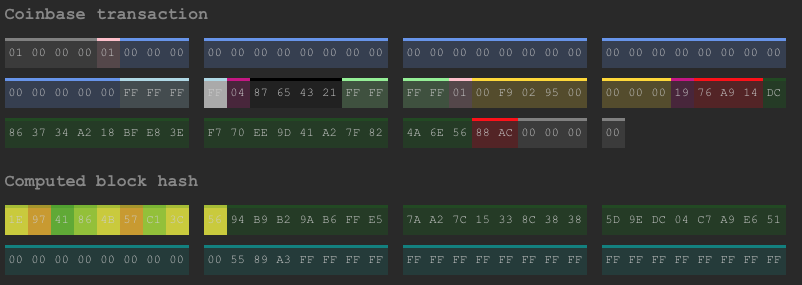
\includegraphics[width=\linewidth]{latex-vorlage_v1.5/graphics/Bildschirmfo.png}
    \caption[Screenshot from the "Blockchain Reader" mining simulator.]{Screenshot from the "Blockchain Reader" mining simulator.\protect\footnotemark}
    \label{fig:BlockchainReader}
\end{figure}
\footnotetext{Taken from \cite{JornCYoghBlockchainReader2017}}

\paragraph{Learn Me a Bitcoin} This website focuses on explaining the essential components of Bitcoin Core by letting the user drill down into different aspects of the blockchain. All primary components of a blockchain are present: the user may inspect a node, its memory pool, the blockchain (and every block in it), the structure of a specific block, the difficulty, the block reward, a specific transaction or a specific address. It also offers a guide and a glossary which explain the fundamental concepts and terms in plain text (with images) in a comprehensive and easy to understand manner. In addition to this, the website includes a number of tools which elaborate on underlying concepts such as hash functions and block headers. Overall, the project is well structured and covers the basic principles of the bitcoin blockchain. It explains all topics in an accessible manner, but due to the unstructured approach that lets the user drill down to their liking, some information might be missed by accident. The additional guide and glossary, however, solve this flaw. Regarding the artifact, this website offers a good insight into how the different concepts should be connected with each other, but it lacks a structured approach of introducing the concepts in the first place.\footcite[Cf.][]{WalkerLearnmeBitcoin2016}

\paragraph{Blockchaindemo.io and Coindemo.io} These two projects, both developed by Sean James Han, offer a more structured approach to explaining the concepts of a) a blockchain and b) bitcoin. The user is guided with bubbles of explanatory text to interact with the application (e.g., adding nodes to the network, creating a block or mutating a transaction). Blockchaindemo is the basis for the coindemo application because the latter focuses more on transactions, fees, and mining rewards whereas the first focuses on blocks, hashes, and the P2P network. Both web pages are accompanied by a blog post that explains key concepts and terms in more detail. However, the explanations are not as detailed as the guide in "Learn me A Bitcoin".\footcites[Cf.][]{HanHowdoesblockchain2017}[cf.][]{HanBlockchainDemo2017}[cf.][]{HanHowdoesbitcoin2017}[cf.][]{HanCoinDemo2017}

\paragraph{CoinViz} Students of UC Berkeley created this website as part of their Information Visualization course. It is aimed at people with very little to no knowledge about bitcoin and offers short (approximately one sentence long) explanations about physical make-up of the network, the network activity, its size and bitcoin's price. In comparison to the previous projects, the visualizations, presented in figure \ref{fig:CoinViz}, are less advanced and offer only little new knowledge on how the technology works.\footcite[Cf.][]{GiudiciCoinViz2016}

\begin{figure}
    \centering
    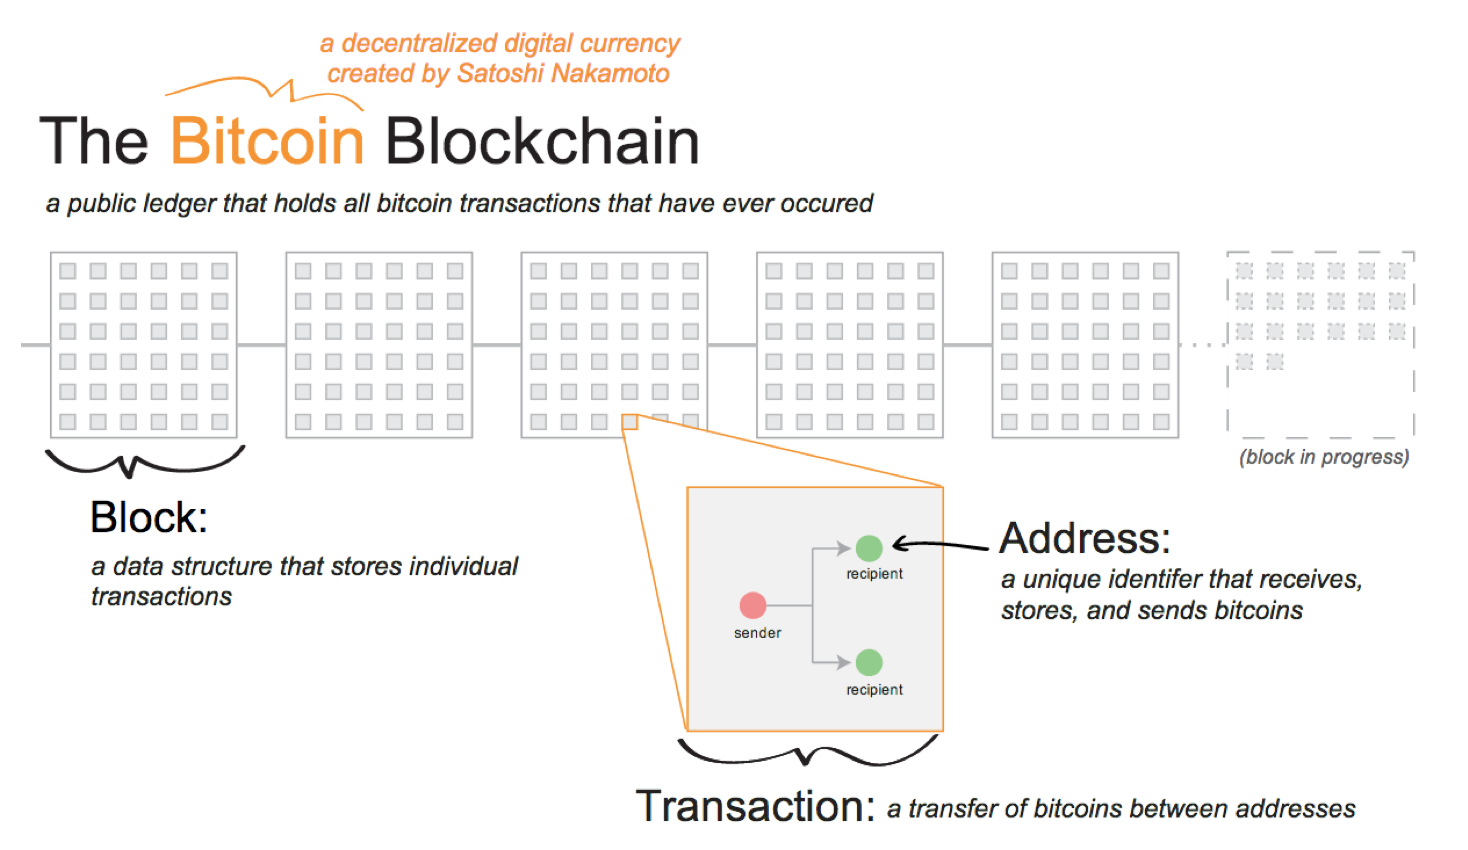
\includegraphics[width=\linewidth]{latex-vorlage_v1.5/graphics/CoinViz.png}
    \caption[CoinViz visualization of the bitcoin blockchain.]{CoinViz visualization of the bitcoin blockchain.\protect\footnotemark}
    \label{fig:CoinViz}
\end{figure}
\footnotetext{Taken from \cite{GiudiciCoinViz2016}}

\paragraph{Symphony of Blockchains} The project of IOHK, the company behind the blockchain implementation Cardano and RSCoin, has produced a 3D visualization of the bitcoin blockchain. The blocks are represented in a chronological funnel which, when interacted with, move and expand. Each block may be opened to present more detailed information regarding its size, date of publication, number of transactions, input and output values as well as a presentation of the Merkle tree, which is under-laid with harmonic sounds. The user is free to scroll through the funnel, representing the time flow and may click any block that is of interest. The visualization is aesthetic and meditative. It should be conceived as an art project rather than a blockchain demonstration. From this point of view, it is understandable how this project only superficially covers the blockchain technology (concepts such as transactions, distributed system, and cryptography are not mentioned) and puts more focus on the beauty of its visualization.\footcite[Cf.][]{IOHKSymphonyBlockchains2018} 

Overall, each of the presented projects offers a different approach to visualizing (and explaining) the blockchain technology. It is interesting to note that the majority focuses on the bitcoin blockchain, although the prevalence of bitcoin in the media (it is the most widely known example of a blockchain) may explain this relation.\footnote{This statement refers to the difference of Google search results for "blockchain": 24.200.000 and "bitcoin": 88.600.000. Search date 18th March 2018}

The blockchaindemo, coindemo and the symphony of blockchain projects are the most visually appealing visualizations, as the user interface is well constructed and of high quality. The projects follow the approach of a tutorial, guiding the user through the different concepts instead of letting them decide which concepts they would want to explore.

This section has treated existing approaches to blockchain visualizations and explanations. In combination with the insight derived from the expert interviews, the requirements elicitation phase is completed. The information now needs to be analyzed more thoroughly, and the requirements need to be formally specified. This is the objective of the following chapter.